% BU ECE template for MS thesis and PhD dissertation.
%
%==========================================================================%
% MAIN PREAMBLE 
%==========================================================================%
\documentclass[11pt,letterpaper]{report}          % Single-sided printing for the library
%\documentclass[12pt,twoside]{report} % Double-sided printing
\usepackage[intlimits]{amsmath}
\usepackage{amsfonts,amssymb}
\DeclareSymbolFontAlphabet{\mathbb}{AMSb}
\usepackage[square,numbers]{natbib}
% \usepackage{apalike}
\usepackage{float}
\usepackage[bf]{caption}       
\setcaptionmargin{0.5in}
\usepackage{fancyhdr}
%\usepackage{fancyheadings}
\usepackage{fancybox}
\usepackage{ifthen}
\usepackage{bu_ece_thesis}
\usepackage{url}
\usepackage{lscape,afterpage}
\usepackage{xspace}
\usepackage{epstopdf} 
\usepackage{subfig}
\usepackage{listings}
%\documentclass[10pt]{•}
%==========================================================================%
%%% graphicx and pdf creation
\usepackage{graphicx}
\usepackage{appendix}
\usepackage{hyperref}
%\usepackage{psfrag}
%\DeclareGraphicsExtensions{.eps}   % extension for included graphics
%\usepackage{thumbpdf}              % thumbnails for ps2pdf
%\usepackage[ps2pdf,                % hyper-references for ps2pdf
%bookmarks=true,%                   % generate bookmarks ...
%bookmarksnumbered=true,%           % ... with numbers
%hypertexnames=false,%              % needed for correct links to figures !!!
%breaklinks=true,%                  % breaks lines, but links are very small
%linkbordercolor={0 0 1},%          % blue frames around links
%pdfborder={0 0 112.0}]{hyperref}%  % border-width of frames 
%                                   % will be multiplied with 0.009 by ps2pdf
%\hypersetup{
%  pdfauthor   = {Joe Graduate <joe.graduate@bu.edu>},
%  pdftitle    = {dissertation.pdf},
%  pdfsubject  = {doctoral dissertations},
%  pdfkeywords = {mathematics, science, technology},
%  pdfcreator  = {LaTeX with hyperref package},
%  pdfproducer = {dvips + ps2pdf}
%}
%==========================================================================%
% customized commands can be placed here
%\newcommand{\figref}[1]{Figure~\ref{#1}}
%\newcommand{\chapref}[1]{Chapter~\ref{#1}}
%\newcommand{\latex}{\LaTeX\xspace}
%==========================================================================%

%==========================================================================%
% BEGIN
%==========================================================================%
\begin{document}

% The preliminary pages
\include{0_Prelim/prelim}        
\cleardoublepage

% -------------------------------------
% CHAPTER 1: INTRODUCTION
% -------------------------------------
\chapter{Introduction}
\label{chapter:Introduction}
\thispagestyle{myheadings}

\section{Problem Description}
\label{sec:history}

Many of popular open source cluster computing frameworks for large scale data analysis, 
such as Hadoop and Spark, allow programmers to define objects in a host languages, such as Java.
The objects are then managed in RAM by the language and its runtime, Java Virtual Machine 
in the case of Java and Scala. Storing objects in memory enables machine to process iterative computation. 
One of the fundamental tasks for recent big data analysis is analysis using Machine Learning Algorithms, 
which require iterative process. As the amount of data increases, memory is required to keep many objects. 
Therefore, memory management plays a critical role in this task. 

Memory management in Java and Scala is performed by garbage collection. 
The garbage collection brings a significant advantage for programmers by removing responsibility
for planning memory management by themselves. Instead, JVM monitors the state of memory and performs garbage
collection at certain points. However, these monitoring and auto-execution of garbage collection cost additional 
computation and might consume computation resources which should be used for data processing. This can significantly decrease performance of the computation. 

In contrast, memory management in system language, such as C++, relies on programmers’ decision for when to allocate and deallocate memory. 
The functions, malloc/free consume most of the memory management. Proper implementation of system language for big data processing can be overperform the implementation in host language.
Nevertheless, implementing C++ performing proper memory management and guaranteeing security can be unproductive and complicated. 

Considering the issue of memory management, we introduce solution based on unique memory management methods implemented in Rust, ownership and borrowing.
This unique concepts in Rust secure codes and perform memory management without monitoring memory or calling functions. We introduce implementations of
machine learning algorithms in both Java and Rust to assess performances of each memory management system for iterative big data processing tasks.


\section{Memory Management in Rust}
\label{sec:history}

Each value in Rust has a variable called its owner. This owner has information about the value, such as location in memory, 
length and capacity of the value. This owner can live on the scope associated with its life time. When the owner goes out of it’s scope, 
the value will be dropped. When a value already assigned to a variable is assigned to another variable, if the value is allocated 
on heap its information is copied to the new owner and drop the old owner disabling old variable. Similar thing happens when we pass variable to parameter of function. 
After passing a variable to a parameter, all the information is copied to new owner through the parameter and old owner is no longer available. 
The new owner can only live in the function and the object will be dropped. In this case, we have no longer access to the object after the function. 
To avoid this, Rust has a concept called borrowing. We can set reference for the parameter of function and use the reference for operation within function and drop the reference, 
but not the ownership. 


\section{Spark and RDD Catching}
\label{sec:history}

Spark is one of the most used big data computing framework. Spark uses Resilient Distributed Datasets (RDDs) which implement in-memory data structures 
used to cache intermediate data across a set of nodes. This enables multiple rounds of computation on the same data, which is required for machine learning 
and graph analytics iteratively process the data. 

In RDD caching, there are different stages of caching, such as MEMOR\_YONLY and DISK\_ONLY. 
Currently, for very large data sets, we need to pay attention to garbage collection (GC) and OS page swapping overhead, 
because these could degrades execution time significantly. Therefore, DISK\_ONLY RDD caching can be better configuration in this case. 
However, writing and reading intermediate data among desk and memory could have bad effects for execution time, due to need of serialization and deserialization. 

\section{BLAS LAPACK}
\label{sec:history}

Basic Linear Algebra System (BLAS) is a linear algebra library written in Fortran. This library includes basic linear algebra functionality such as matrix addition 
and dot product. LAPACK is developed on BLAS and has advanced functionality such as LU decomposition and Singular Value Decomposition (SVD). These library optimize 
hardware use for linear algebra operation so they are hardware dependant.

Linear algebra library used for Spark is netlib-java, which is a Java wrapper library for Netlib, C API of BLAS and LAPACK. The reason why the developers addressed 
to use this package is that the BLAS and LAPACK are already bug free and implementing linear algebra library from scratch can usually buggy. 

However, the main advantage of use of BLAS and LAPACK is system optimized implementation. So if we implement original Fortran linear algebra library, 
it cannot perform as well as BLAS and LAPACK. And the performance would not be such different from one of implementation in Java or Rust.  If we want to test only memory management between Rust and Java,
 it can be enough implementation of linear algebra operation from  pure Java and Rust sacrificing the best performance taking advantage of system optimization. My concern is implementing linear algebra operation
  from scratch can be buggy and cause a lot of problems when we test on machine learning algorithms.

\cleardoublepage

% -------------------------------------
% CHAPTER 2: THE BODY OF THESIS
% -------------------------------------
\include{2_RelatedWork/RelatedWork}
\cleardoublepage

% -------------------------------------
% CHAPTER 3: THE BODY OF THESIS
% -------------------------------------
\chapter{Experiment}
\label{chapter:body}
\thispagestyle{myheadings}

% set this to the location of the figures for this chapter. it may
% also want to be ../Figures/3_Body/ or something. make sure that
% it has a trailing directory separator (i.e., '/')!
\graphicspath{{3_Body/Figures/}}

\section{Concept}
\label{sec:history}
\subsection{Type of Variable}
\label{sec:history}
In Rust, there are three variable types: owner, reference, and slice (only for sequence of values). 
A developer is sometimes forced to use specific variable types. For example, some of methods are only implemented to specific variable types.
However, one can select any variable types for operation in most case.

These variables have different memory representation shown in Figure~\ref{fig:own_ref_slice}.
The owner has a pointer pointing to the memory address of sequence values, length of the values, and capacity allocated to store additional values. 
Reference and Slice are variables borrowing value owned by other variable. The reference is a pointer that points to the owner. 
The slice is a pointer that points to memory address of sequence values. It has value such as length of sequence values stored in the memory. 
Since they have different memory representation, an assumption is that it takes different time to access to the contents of the memory among these pointer types.
We examine this by constructing complex objects whose fields are these variable types. The details are explained in section 3.2.

\begin{figure}[htb]
    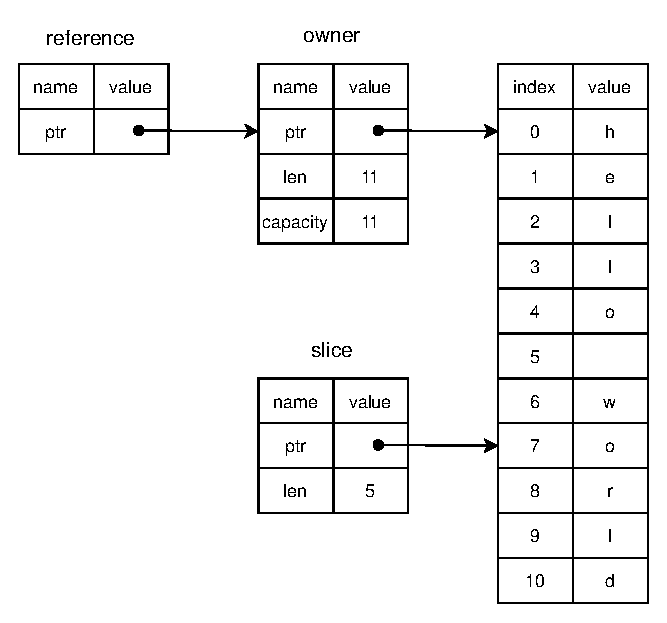
\includegraphics[width=10cm]{own_ref_slice.eps}
    \caption{Memory Representation of Owner, Reference, and Slice Type}
    \label{fig:own_ref_slice}
\end{figure}

\subsection{Reference Count}
\label{sec:history}
Reference is useful to avoid movement of ownership. However, one needs to track its lifetime and explicitly includes it in code, 
because Rust compiler cannot infer it. This can be another encumbrance. We can instead acquire multiple owners to single value by using Reference Counting (Rc). 
By leveraging Rc, a value can be shared like what borrowing plays the role in Rust programming. 

The difference is that Rc checks number of owner pointing to the actual data and makes sure the data is not deleted 
until all the owners are dereferenced. Using Rc is sometimes preferable approach for developers especially when lifetime planning is extremely difficult.
However, the possible problem regarding to Rc is the cost for tracking the number of references. 
Having this assumption, an experiment is conducted to examine difference of runtime performance of dropping reference and Rc. 
This is explained in section 3.2.

\subsection{Multithreading}
\label{sec:history}
In Rust programming, writing concurrent code is relatively easy. The care Rust takes with reference, mutability, and lifetimes is valuable enough in single-threaded programs, 
but it also is in concurrent programming. Rust has tools to write concurrent code, such as threads, locks, atomic reference. 
Therefore, one can implement various concurrent codes for the same purpose with different memory management strategies. 
The most ubiquitous tool used in Rust concurrent code is Atomic Reference Counting (Arc). 

Arc is a simple interface that allows threads to share data. Arc allows multiple variable to have ownerships of a particular value similarly to Rc, 
but also supports atomic feature enabling the ownerships exist in different threads. 
In many situation where developer write a multithreading code, the deletion of Arc happens significant amount of times. 
Similarly to Rc, our assumption is that deletion of Arc has also overhead when we compare to normal reference. 
To assess runtime performances of algorithm with Arc vs normal reference, we implement merge-sort algorithm in two different ways. 

\subsection{Tree-aggregate}
\label{sec:history}
Finally, we implement some of algorithm common in Big Data processing. One of them is tree-aggregate.

Tree-aggregate is a communication patten heavily used for Machine Learning algorithm in Spark (MLlib). 
The topology of aggregation patterns in Apache Spark are shown in Figure~\ref{fig:aggregationk_patttern}. 
In the traditional aggregation function in Spark, results of aggregation in all executor clusters are sent to the driver. 
That is why this operation suffers from the CPU cost in merging partial results and the network bandwidth limit.
Tree-aggregate is a communication pattern which overcomes these problems by breaking aggregate operation in multi-level represented like tree structure.

Spark generates intermediate objects from RDDs. In Tree-aggregation, aggregated HashMap like data structure is created in each thread or node. 
When it aggregates objects in RDD, copy of objects in source vector should be performed to construct intermediate aggregated data structure.
In another way, one can use reference to the objects to perform aggregation instead of copying the values themselves.
In Rust, we can clone or get Arc (Rc if in single thread) of objects to implement these operations.

Since Tree-aggregation algorithm generates and deletes a lot of intermediate data structures, 
how the data structures are constructed and how they are deallocated is important concern in memory management in this algorithm.
In our experiment, tree-aggregation algorithms are examined in multi-threading. The detail is described in section 3.2.

\begin{figure}[htb]
    \begin{minipage}[t]{0.5\linewidth}\centering
        \includegraphics[width=5cm]{normal_agg.eps}
        \medskip
        \centerline{(a)}
        \end{minipage}\hfill
        \begin{minipage}[t]{0.5\linewidth}\centering
        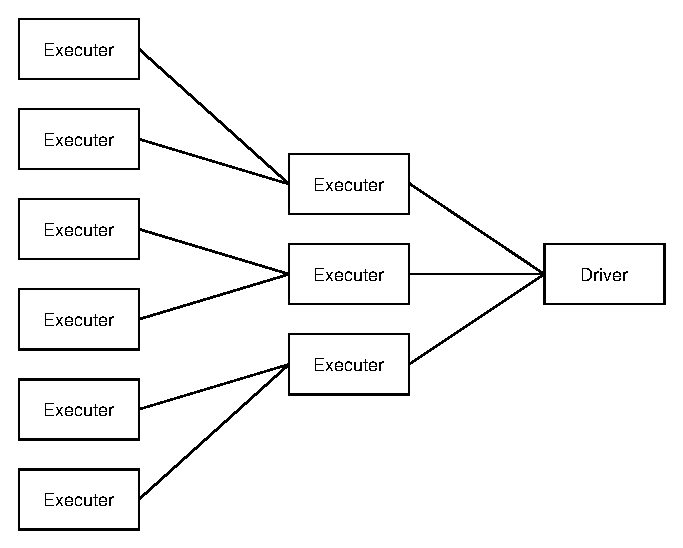
\includegraphics[width=7cm]{tree_agg.eps} 
        \medskip
        \centerline{(b)}
    \end{minipage}\hfill
    \caption{Representation of aggregation strategies in Apache Spark: (a) Traditional Aggregation, (b) Tree Aggregation}
    \label{fig:aggregationk_patttern}
\end{figure}

\subsection{K-Nearest-Neighbors}
\label{sec:history}
The other algorithm common in Big Data processing is K-nearest-neighbors (KNN). KNN is a traditional Machine Learning algorithm which classify targets into categories. 
In training KNN, it simply stores all available training data without calculation. At prediction phase, targets are given and similarity measures are calculated. 
Based on these similarities, the algorithm selects \(K\) (user-defined number) training observations similar to the each target. 
Then, it checks corresponding categories of the \(K\) observations to determine predicted category. 

In brute force algorithm, KNN calculates similarity measures for all combinations among training and testing observations. 
If training data has \(N\) observations and test data has \(M\) observations, KNN needs to calculate \(N \times M\) similarity measures. 
Sort or binary heap can be used to select the \(K\) most similar training observations.

In our experiment, KNN algorithms performs document classification and implemented in multithread. 
There are three phases in our algorithm: preprocessing, query, and combine phase. 
In preprocessing phase, the algorithm calculates Term-frequencies (Tfs) to generate numeric feature vectors and matrices. 
In query phase, similarity measures are calculated and \(K\) nearest neighbors are selected. 
For similarity measure, our choice is cosine similarity(~\ref{eq:cosine}). 
In combine phase, results of query phase are gathered and combined from each threads.

\begin{equation} \label{eq:cosine}
    Cos(\vec{x}, \vec{t})
     = \frac{\sum_{i=0}^{n} (x_i t_i)}{\sqrt{\sum_{i=0}^{n} x_i^2}\sqrt{\sum_{i=0}^{n} t_i^2}}
\end{equation}

Even though preprocessing phase is not specific process for KNN algorithm, 
it is common in algorithms used in Natural Language Processing. Therefore, better memory management strategy should be applied in this preprocessing phase.
This preprocessing generates many intermediate data structures and copies of String elements are used in these data structure again and again. 
We can again either clone or get Arc of String. 

Our KNN algorithms are implemented with batch processing. In query phase, we control batch size to examine how size of objects allocated simultaneously in memory has impact to algorithm's runtime performance.
The detail implementation is explained in section3.2.

\subsection{Complex Objects}
\label{sec:history}
To conduct experiments for above concepts, we use the 4 types of complex object: CustomerOwned, CustomerBorrowed, CustomerSlice, and CustomerRc. 
These object contains other type of object: OrderOwned, OrderBorrowed, OrderSlice, and OrderRc.
The representation of these objects are shown in Figure~\ref{fig:customer} and Figure~\ref{fig:order}. 
Three Customer objects have 15 fields: 3 fields for i32, 3 fields for f64, 8 fields for String, and 1 field for Order object.
All of fields of CustomerOwned and OrderOwned are owned by the object. On the other hand, fields of CustomerBorrowed, CustomerSlice, OrderBorrowed, and OrderSlice are borrowed. 
Reference of slice of values are used as the fields and owner of actual values are stored differently in source Vec. 
CustomerRc acquires Rc of values used for its fields from the source Vec.

\begin{figure}[htb]
    \begin{minipage}[t]{0.2\linewidth}\centering
        \begin{lstlisting}
            struct CustomerOwned {
                key: i32,
                age: i32,
                num_purchase: i32,
                total_purchase: f64,
                duration_spent: f64, 
                duration_since: f64,
                zip_code: String,
                address: String,
                country: String,
                state: String,
                first_name: String,
                last_name: String,
                province: String,
                comment: String, 
                order: OrderOwned
            }
        \end{lstlisting}
      \medskip
      \centerline{(a)}
    \end{minipage}\hfill
    \begin{minipage}[t]{0.6\linewidth}\centering
        \begin{lstlisting}
            struct CustomerBorrowed<'a> {
                key: &'a i32,
                age: &'a i32,
                num_purchase: &'a i32,
                total_purchase: &'a f64,
                duration_spent: &'a f64, 
                duration_since: &'a f64,
                zip_code: &'a String,
                address: &'a String,
                country: &'a String,
                state: &'a String,
                first_name: &'a String,
                last_name: &'a String,
                province: &'a String,
                comment: &'a String, 
                order: &'a OrderBorrowed<'a>
            }
        \end{lstlisting}
      \medskip
      \centerline{(b)}
    \end{minipage}
    \begin{minipage}[t]{0.2\linewidth}\centering
        \begin{lstlisting}
            struct CustomerSlice<'a> {
                key: &'a i32,
                age: &'a i32,
                num_purchase: &'a i32,
                total_purchase: &'a f64,
                duration_spent: &'a f64, 
                duration_since: &'a f64,
                zip_code: &'a str,
                address: &'a str,
                country: &'a str, 
                state: &'a str,
                first_name: &'a str,
                last_name: &'a str,
                province: &'a str,
                comment: &'a str,
                order: &'a OrderSlice<'a>
            }
        \end{lstlisting}
      \medskip
      \centerline{(c)}
    \end{minipage}\hfill
    \begin{minipage}[t]{0.6\linewidth}\centering
        \begin{lstlisting}
            struct CustomerRc {
                key: Rc<i32>,
                age: Rc<i32>,
                num_purchase: Rc<i32>,
                total_purchase: Rc<f64>,
                duration_spent: Rc<f64>,
                duration_since: Rc<f64>,
                zip_code: Rc<String>,
                address: Rc<String>,
                country: Rc<String>,
                state: Rc<String>,
                first_name: Rc<String>,
                last_name: Rc<String>,
                province: Rc<String>,
                comment: Rc<String>,
                order: Rc<OrderRc>
            }
        \end{lstlisting}
      \medskip
      \centerline{(c)}
    \end{minipage}\hfill
    \caption{Representation of Customer objects Whose fields are different variable type: (a) CustomerOwned struct whose fields are all owned 
    (b) CustomerBorrowed struct whose fields are borrowed with reference (c) CustomerSlice struct whose fields are borrowed with slice for sequence value, otherwise reference}
    \label{fig:customer}
 \end{figure}

 \begin{figure}[htb]
    \begin{minipage}[t]{0.2\linewidth}\centering
        \begin{lstlisting}
            struct OrderOwned {
                order_id: i32,
                num_items: i32, 
                payment: f64,
                order_time: f64,
                title: String,
                comment: String
            } 
        \end{lstlisting}
      \medskip
      \centerline{(a)}
    \end{minipage}\hfill
    \begin{minipage}[t]{0.6\linewidth}\centering
        \begin{lstlisting}
            struct OrderBorrowed<'a> {
                order_id: &'a i32,
                num_items: &'a i32, 
                payment: &'a f64,
                order_time: &'a f64,
                title: &'a String,
                comment: &'a String
            }
        \end{lstlisting}
      \medskip
      \centerline{(b)}
    \end{minipage}
    \begin{minipage}[t]{0.2\linewidth}\centering
        \begin{lstlisting}
            struct OrderSlice<'a> {
                order_id: &'a i32,
                num_items: &'a i32, 
                payment: &'a f64,
                order_time: &'a f64,
                title: &'a str,
                comment: &'a str
            }
        \end{lstlisting}
      \medskip
      \centerline{(c)}
    \end{minipage}\hfill
    \begin{minipage}[t]{0.6\linewidth}\centering
        \begin{lstlisting}
            struct OrderRc {
                order_id: Rc<i32>,
                num_items: Rc<i32>,
                payment: Rc<f64>,
                order_time: Rc<f64>,
                title: Rc<String>,
                comment: Rc<String>
            }
        \end{lstlisting}
      \medskip
      \centerline{(c)}
    \end{minipage}\hfill
    \caption{Representation of Order objects Whose fields are different variable type: (a) OrderOwned struct whose fields are all owned 
    (b) OrderBorrowed struct whose fields are borrowed with reference (c) OrderSlice struct whose fields are borrowed with slice for sequence value, otherwise reference}
    \label{fig:order}
 \end{figure}

 \subsection{Wikipedia Data Sets}
 \label{sec:history}
 Wikipedia page data sets are used to perform document classification with KNN. 
 \(10^5\) pages are used for training data set, and 18724 pages are used for target.

 \subsection{Experimental Details}
 Our experiments are run on three types of VM instances on Google Cloud Platform: 
 n1-standard-1 which has 1 vCPU, 3.75 GB RAM, and 10 GB Standard persistent disk, 
 n1-standard-4 which has 4 vCPU, 15 GB RAM, and 10 GB Standard persistent disk, 
 n1-standard-8 which has 8 vCPU, 30 GB RAM, and 10 GB Standard persistent disk,  
 All of the experiments described are performed 5 times. 
 In this thesis, we present the average of 5 separate runs for each experiment.
\clearpage

\clearpage

\section{Evaluation}
\label{sec:history}

\subsection{Experiment for Accessing Object with Different Variable Type}
\label{sec:eval_diffval}
This experiment is conducted to understand two questions. One is how different variable types have impact to runtime performance.
The other is how initialization of Vec size has impact to runtime performance. 
In this experiment, we focus on owner, reference, and slice as a variable of sequence values. 
Since these variables have different memory representation, there might be differences among time for access to actual values of each variables.

To evaluate this assumption, we use the three types of complex object: CustomerOwned, CustomerBorrowed and CustomerSlice. 
At first, we generate source Vecs for all fields, Vecs which contain all elements used for corresponding fields of objects.
For example, all of i32 elements used for key field in 1 million Customer object are stored in Vec$<$i32$>$ with 1 million i32 elements. 
Later, these i32 elements are moved to be owned or borrowed by the object's fields.

Next, 1.5, 1.8, 2.5, 2.8, 3.5, and 3.8 million of Customer objects are created and stored in Vec. 
When a Customer Vec is created, whether size of Vec is initialized is controlled. 
Finally, serialization of Customer object is performed as an operation forcing program to access all of fields in the object.
This serialization is performed each Customer objects in the Vec. We measure total runtime to serialize all of Customer objects 
stored in Vec. 

\subsection{Result}
\label{sec:history}
The result is shown in Figure~\ref{fig:rustaccessinit} and Figure~\ref{fig:rustaccessnoinit}.
Figure~\ref{fig:rustaccessinit} is comparison of the runtime performance among different Customer object types with Vec size initialization.
Figure~\ref{fig:rustaccessnoinit} is comparison in the same set of experiment except Vec size is not initialized. 
The blue, yellow, and green chats represent runtime of access to fields of CustomerOwned, CustomerBorrowed, and CustomerSlice objects respectively.

No matter Vec size initialized or not, differences of runtime for accessing objects are not remarkable among different object types. 
The percent increase in runtime of accessing to fields of from 1.5 to 3.8 million CustomerOwned objects is 121\% if the Vec is initialized, 554\% if the Vec is not initialized.

Considering the differences of percent increase of runtime whether the Vec is initialized or not, 
Figure\ref{fig:init_vs_noinit} the comparison of runtime access to fields of CustomerOwned object with and without Vec Initialization.
For 3.8 million of objects, the difference of runtime to access to the objects is 38745 secounds; program without Vec initialization is 60\% slower than one with the initialization.

\begin{figure}[htb]
    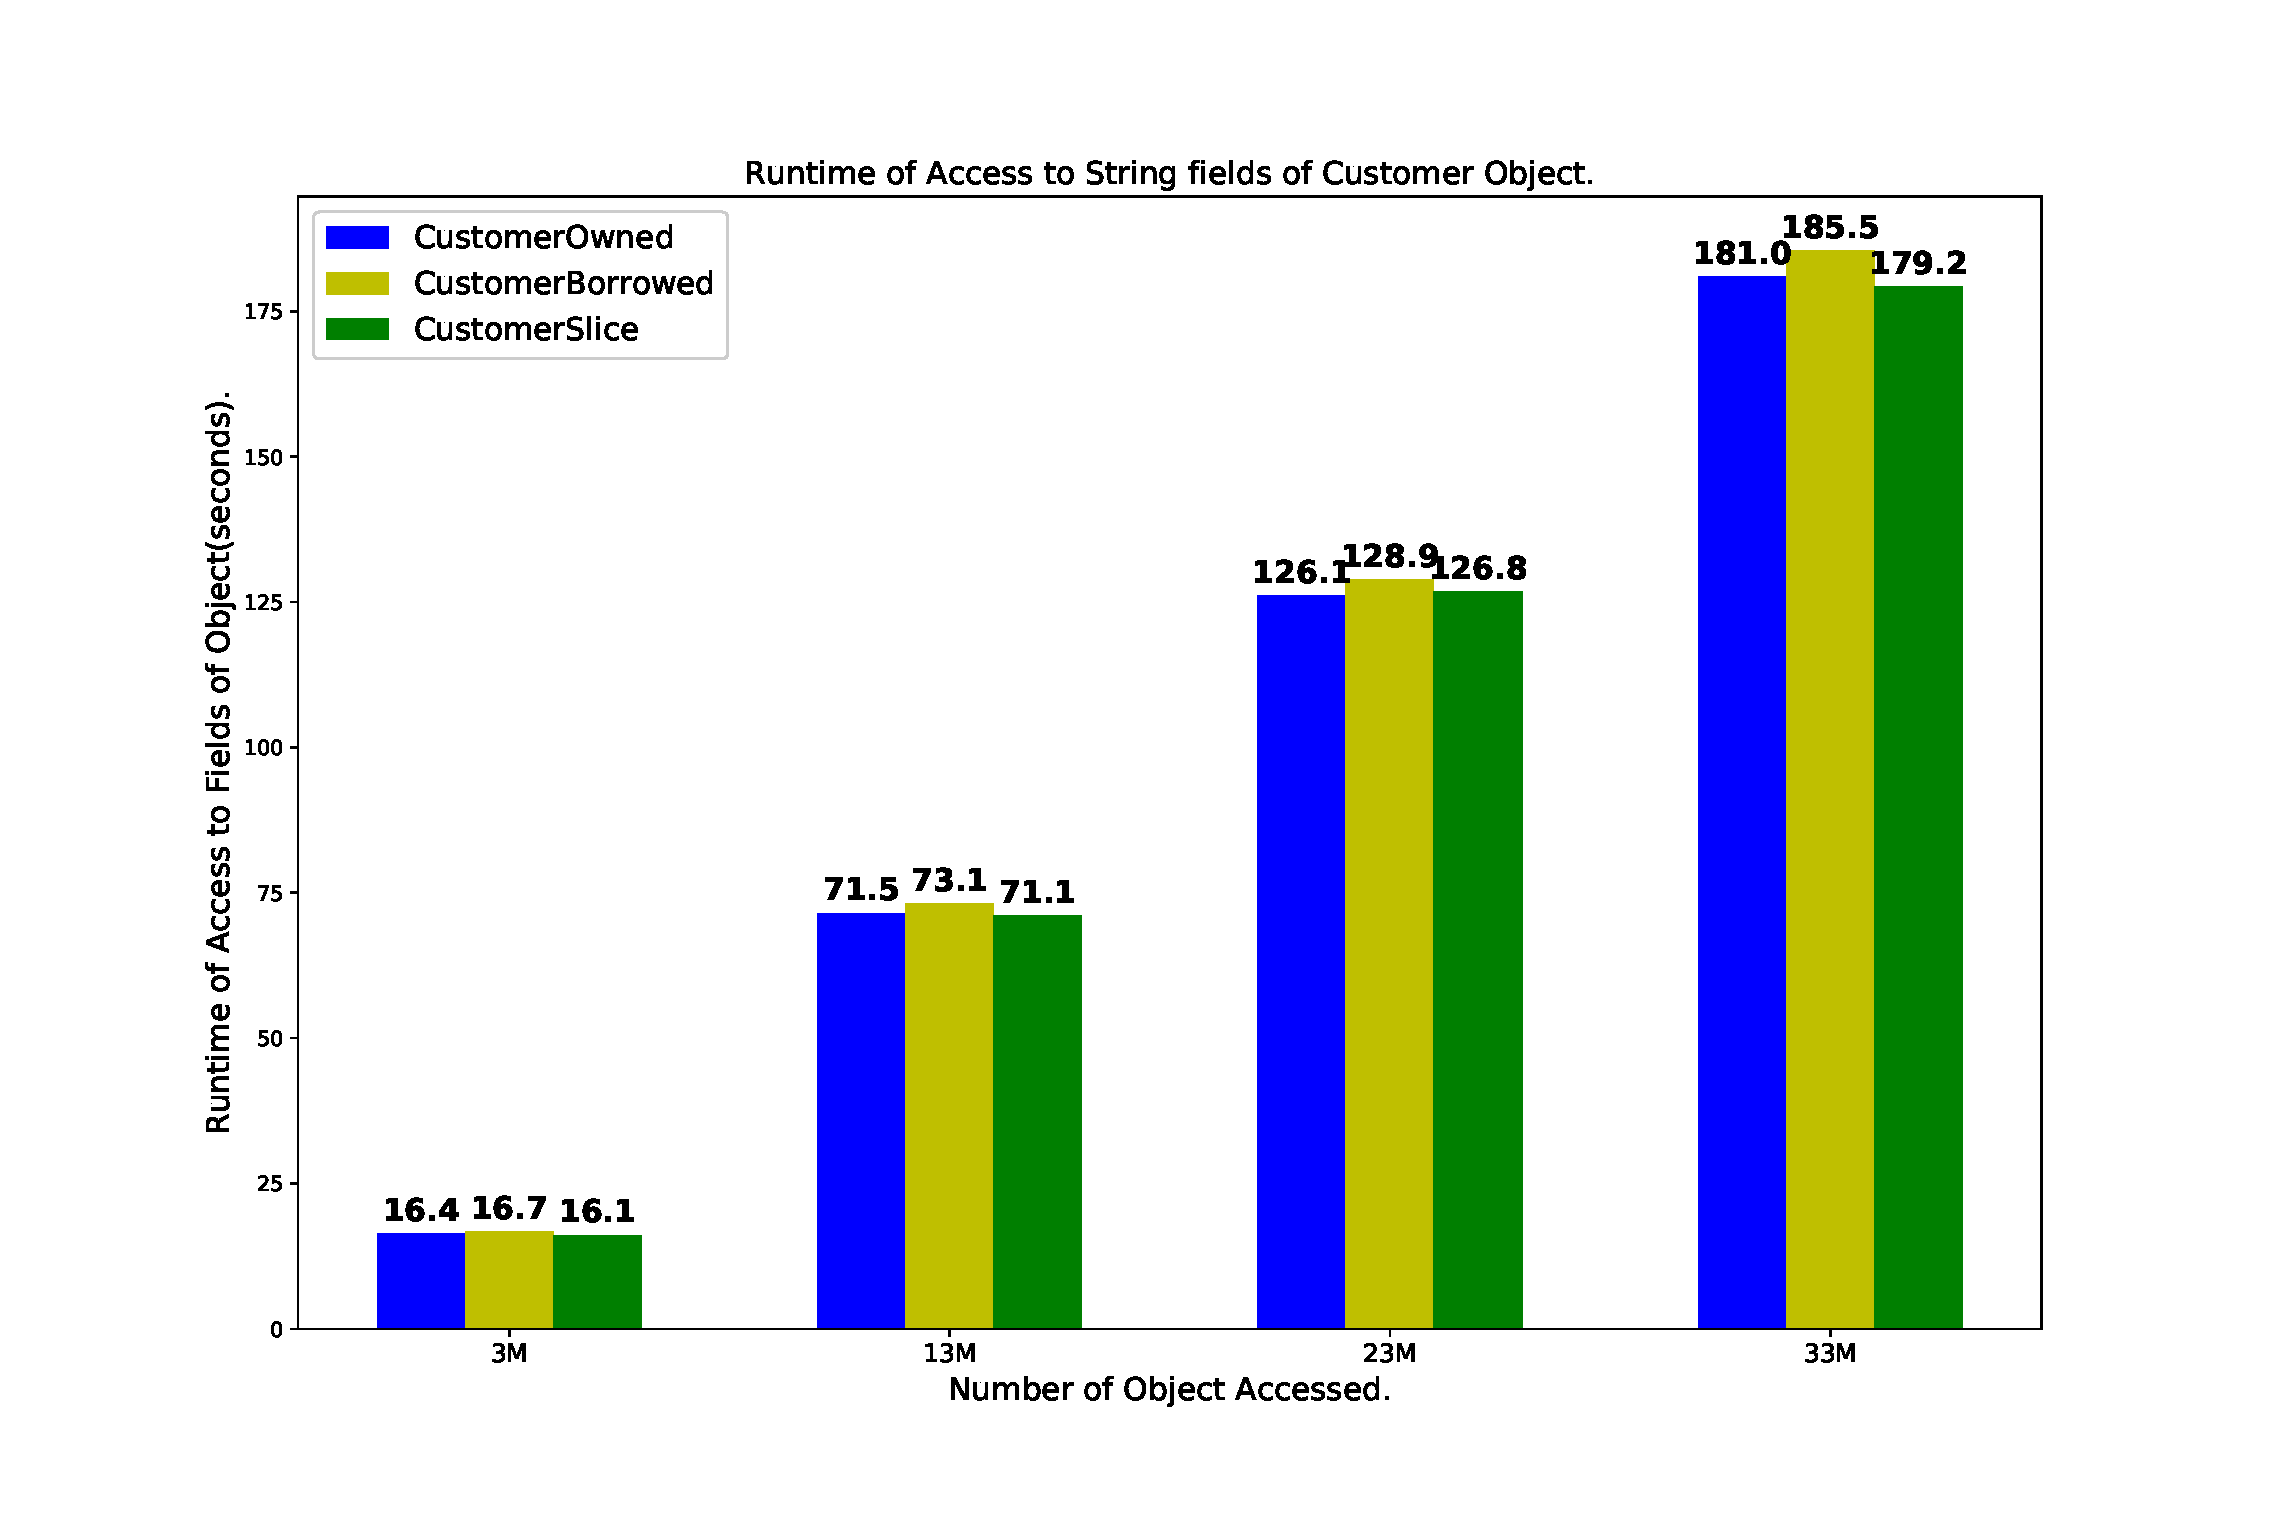
\includegraphics[width=15cm]{rust_access_different_poniter_init.eps}
    \caption{Runtime of Access to Different Pointer Types with Vec Size Initialization}
    \label{fig:rustaccessinit}
\end{figure}

\begin{figure}[htb]
    \includegraphics[width=15cm]{rust_access_different_poniter_noinit.eps}
    \caption{Runtime of Access to Different Pointer Types without Vec Size Initialization}
    \label{fig:rustaccessnoinit}
\end{figure}

\begin{figure}[htb]
    \includegraphics[width=15cm]{rust_access_init_vs_noint.eps}
    \caption{Runtime of Access to Fields of Complex Object with Initialization vs without Initialization}
    \label{fig:init_vs_noinit}
\end{figure}

\subsection{Discussion}
\label{sec:history}
Difference of variable types does not have huge impact to runtime of accessing to actual value.
Even thought owner, reference , and slice have different memory representations, the access time to its value is 
close to each other. As shown in Figure~\ref{fig:own_ref_slice}, the representations of owner and slice are almost identical except slice does not have capacity for values.
Reference is pointer pointing to owner, so it has an additional step to access actual value. 
However, the result shows this additional step does not have huge impact for runtime to access memory region of the value.

Whether initializing Vec size results in disparity of runtime performance to access objects' fields. 
This is because when Vec uninitialized, the elements of Vec are allocated across different virtual memory pages.


\clearpage

\subsection{Assessment of different reference methods in Rust}
\label{sec:eval_refcount}
\subsection{Concept}
The goal of this experiment is to assess efficiency of different reference strategies in Rust, borrowing and reference counting. 

By levaraging reference counting, a value can be shared like what borrowing plays the role in Rust programming. 
The difference is that reference counting checks number of reference pointing to the actual data and makes sure the data is not deleted 
until all the references are dereferenced. Using reference counting is sometimes preferable approach for developers, 
we do not have care about lifetime which is usually troublesome when we use borrowing approach many times in our code. 
However, the possible problem regarding to reference counting is the cost for tracking the number of references. 
Having this assumption, this experiment will show difference of behavior among reference countinig and borrowing.

In this experiment, CustomerBorrowed and CustomerRc in figure are used to see difference of dropping time among borrowing and reference counting. 
In the CustomerRc and OrderRc struct, all fields take reference counting (Rc$<$T$>$). Similaly to the experiment in the last section, 
vectors of CustomerRc and CustomerBorrowed are created and droped the elements one by one. 

The result shows significant difference of dropping time among the two objects; deletion of CustomerRc is much slower than CustomerBorrowed. 
This is because reference counters which are feilds of CustomerRc have to check the number of reference pointing to the actual content and decide 
deallocate the memory or not. However, memory management and lifetime strategy of borrowing is already determined at compile time.


In this experiment, an assessment is conducted to valify whether there is difference between behavior of borrowing and reference counting. 
These two methods can be used in similar situation. Especially, when we want reference to an original variable and keep the original variable until all of references are dereferenced, 
we can have reference with both storategies, borrowing and reference counting. One advantage of using reference counting is that we do not have to pay attention to lifetime.
However, the assumption here is that use of reference counting might be computationally expenesive than borrowing, because reference counting has to track the number of reference pointing to the value. 
Considered this assumption, we assess difference of time for dropping reference using borrowing and reference counting strategies. 

Similally to the last section, we implement struct whose fields are borrowing reference and reference counting and measure the time to drop the struct. 


\subsection{Result}
The result shows the time to drop borrowing reference is significatly faster than reference counting. This says that we should use borrwoing storategies whenever high performance computation is critical.
\begin{figure}[htb!]
    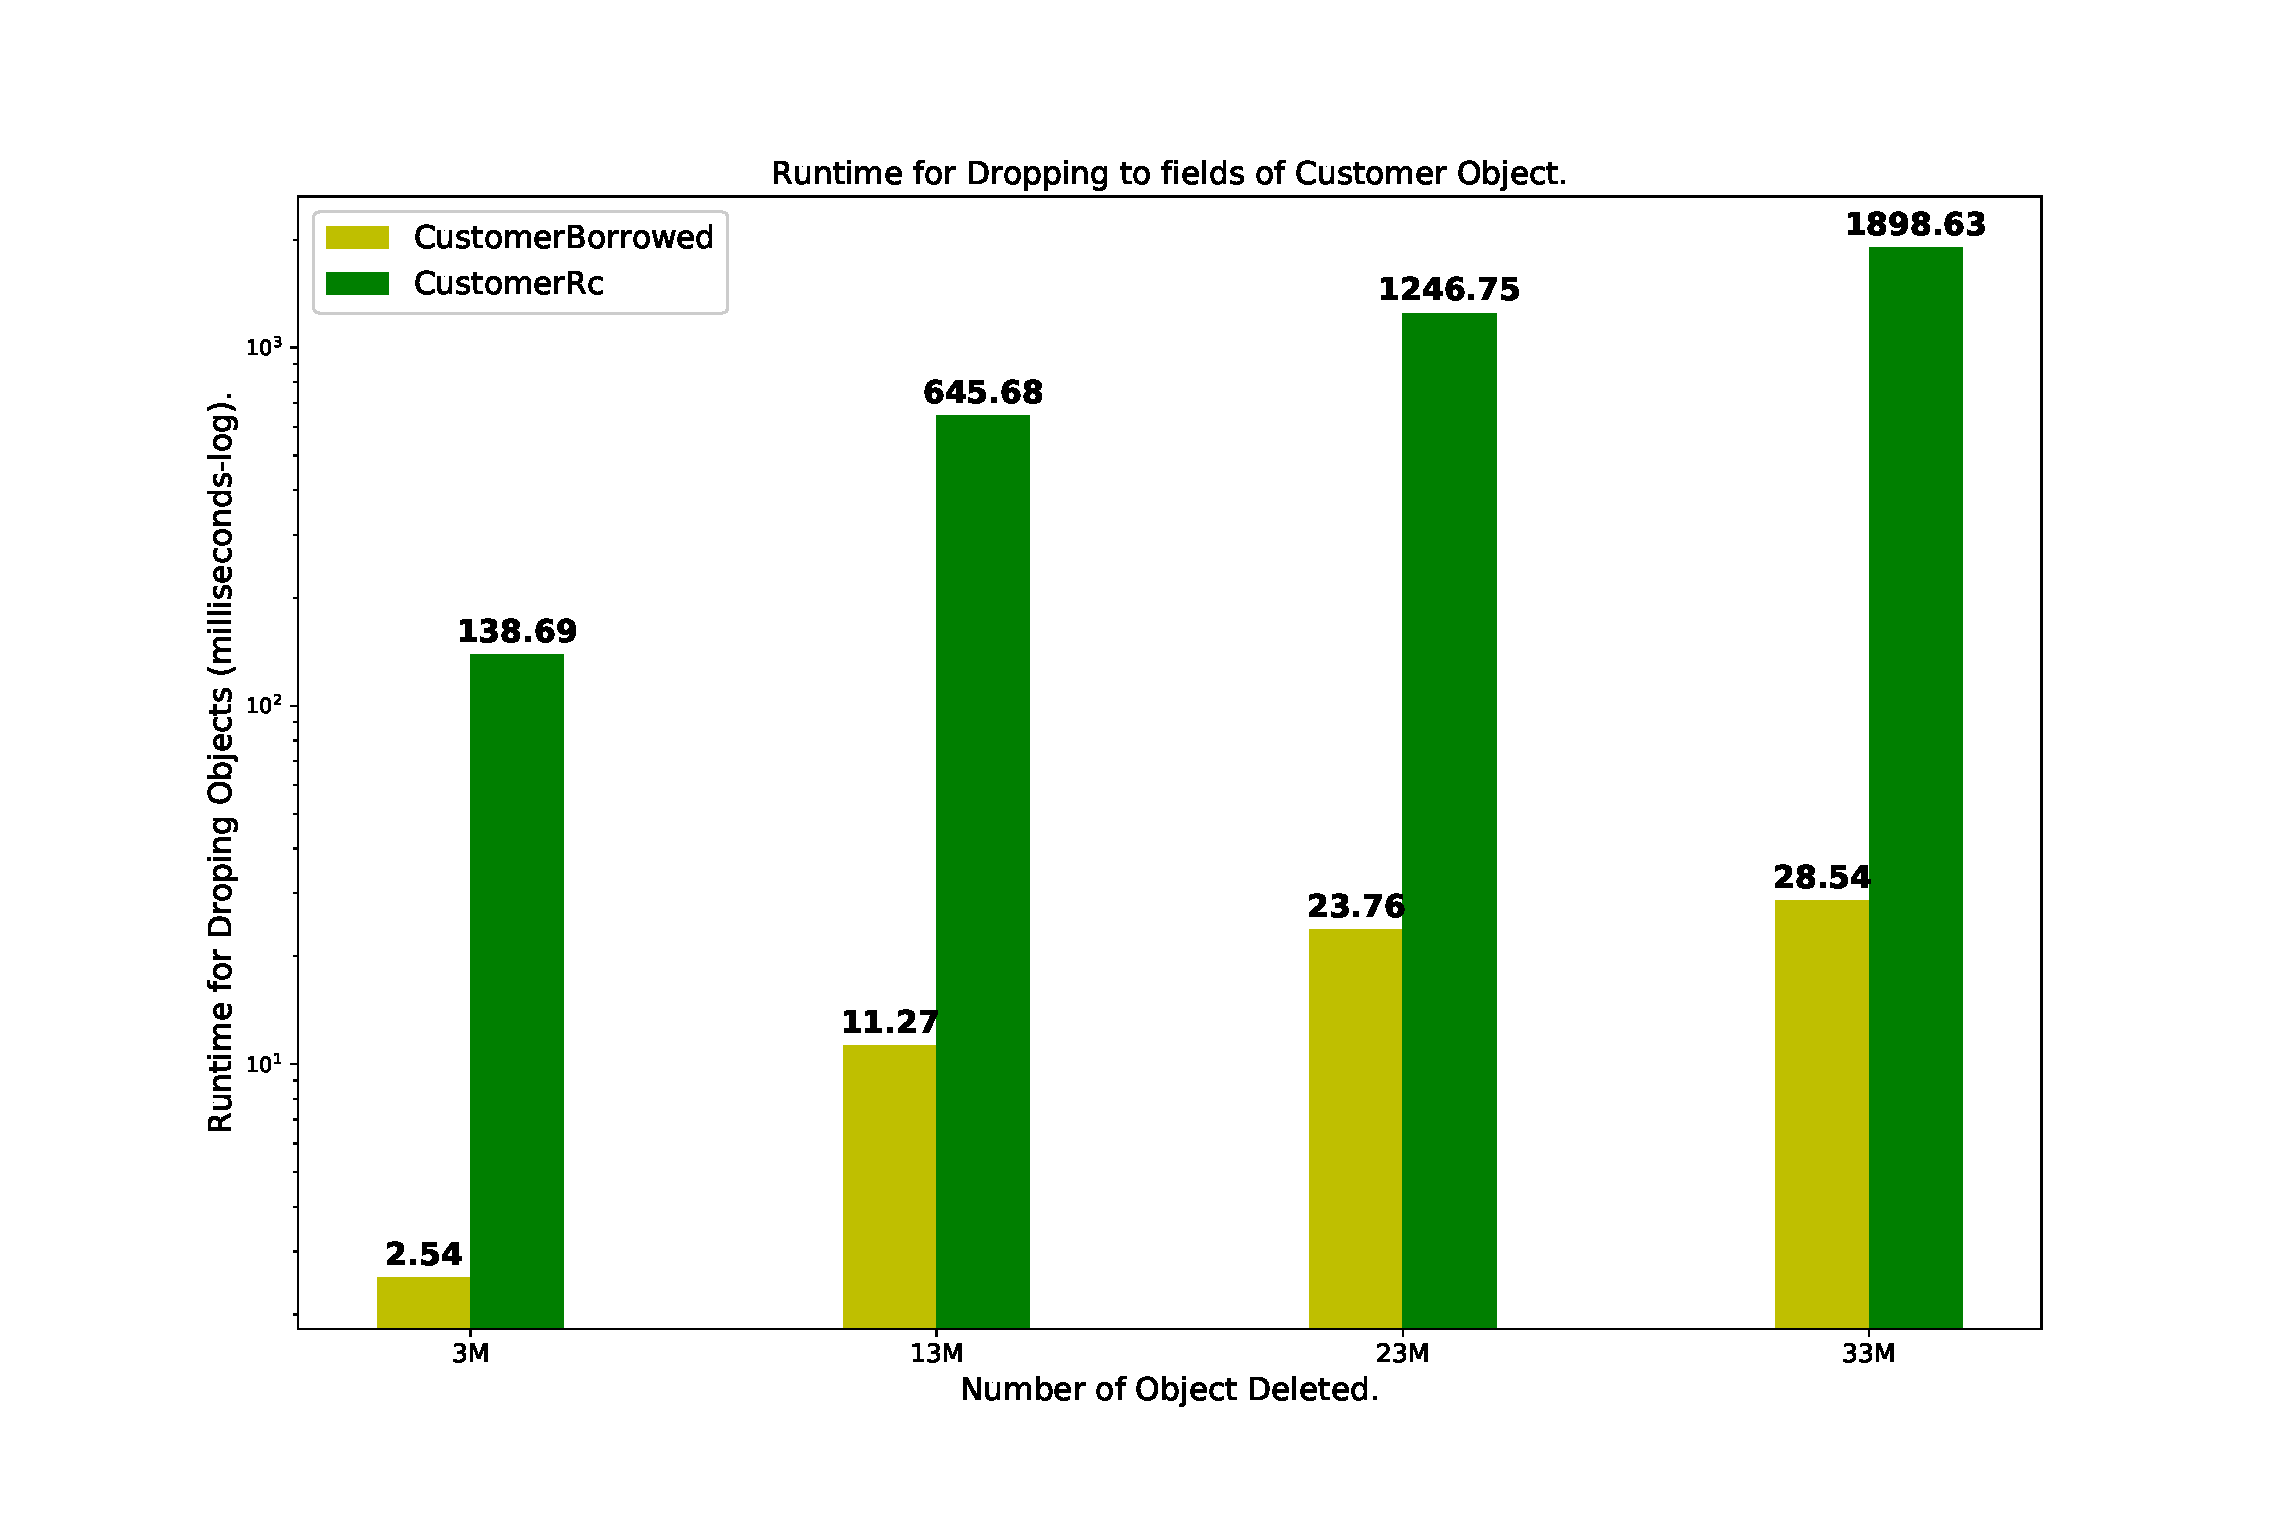
\includegraphics[width=15cm]{rust_droptime_borring_rc.eps}
    \caption{Runtime for Droping to fields of Customer Object}
    \label{fig:Sampling}
\end{figure}

\subsection{Discussion}

\clearpage

\subsection{Experiment for Merge-sort}
\label{sec:eval_sort}
This experiment is to assess importance of careful memory management in multithreading of Rust. 
We implement merge-sort algorithm in two different ways. One is sharing source vector with Arc. 
The other is passing slice of source vector to child thread. 

Our merge-sort algorithm with vector is implemented with recursion. In these alogorithm, the splitting phase is merely aquiring index of split position, 
not actually splitting the source vector. At merge phase, merge function receives two independent vector and merge these into single new vector.

For sharing data implementaion, channel with sending data is used for multithreading method, because we want to ensure children threads return values before parent thread proceed execution. 
For passing slice implementation, we use scope method to enable children threads to receive reference from their parent ensuring the same purpose of sending data. 

Experiment performed is the comparison among sharing data and passing slice implementations to see the impact of Arc, Atomic reference conuting, to runtime performance.
These two implementations are theoritically the same operations other than using or not using Arc to share data. 
This comparison can effectively show how important careful memory management is in multithreading computation in Rust. 
In another word, how atomic reference counting can cost for computation in Rust programming.

The figure shows the result of 
An atomic reference count of the shareable vector is passed to every recursion steps and 


\begin{figure}[htb]
    \includegraphics[width=15cm]{rust_merge_sort.eps}
    \caption{Runtime of Sortting Elements of Customer Vector}
    \label{fig:Sampling}
\end{figure}



The other is LinkedList implementation other than vector.
The linkedlist implementation is different from another two. This algorithm is inplace sorting so that it does not de/allocate memory during execution. 
The comparison among vector and linkedlist implementations can show trade-off between contiguous memory access and inplace non memory de/allocation. 
Experiment with Java linkedlist implementation can be interesting, because Java GC is severe problem when number of object is large. 
\clearpage

\subsection{Experiment for Tree-aggregation}
\label{sec:eval_treeagg}
Tree-aggregate is a communication patten heavily used for Machine Learning algorithm in Spark (MLlib). 
In the traditional aggregation function in Spark, results of aggregation in all executor clusters are sent to the driver. 
That is why this operation suffers from the CUP cost in merging partial results and the network bandwidth limit.
Tree-aggregate is a communication pattern which overcomes these problems by breaking aggregate operation in multi-level represented like tree structure.

In multi-thread situation, tree-aggregate is just fork-join thread algorithm. We already implemented Merge-Sort algorithm with fork-join. 
If we implement tree-aggregate with multi-thread, the difference is only aggregation and sorting.
\clearpage

% \subsection{Elements Copy and Insertion into Size-initialized Vector in Rust.}
% \label{sec:history}
% In this experiment, four methods are used to insert elements into vector in Rust. One is clone method which performs bitwise deep copy. 
Another is clone\_from which also performs bitwise deep copy, but copies elements of the vector to distination vector rather than 
creating new one. We initialize the distination vector with the same size to the number of elements we insert into it. 
Another is copy\_nonoverlapping function which copies values from source to distination memory region. 
The other is pushing elements of source to distination vector one by one. Insertions of elements with 4 size are conducted 1000000, 1500000, 10000000, 15000000, and, 
their runtimes for each elements type, integer and String are measured. 


The figure shows the result of the experiment. Among the runtime performances of integer insertion for every methods, 
clone, clone\_from, and copy\_nonoverlapping method shows the similar performance. However, the pushing the copy of elements one by one has much slower runtime performance 
compared to the rest. This is because integer elements are allocated contiguously in the memory, so that accessing address of memory by pointer reads some next address. 
This boosts the copy and insertion of elements. 

On the other hand, all of methods show the similar runtime performance in experiment for String object insertion. 
This is because String object is not stored in contiguous memory region. The vector stores pointer to the object and 
process need to access around different memory region again and again to deeply copy the object.

\begin{figure}[htb]
    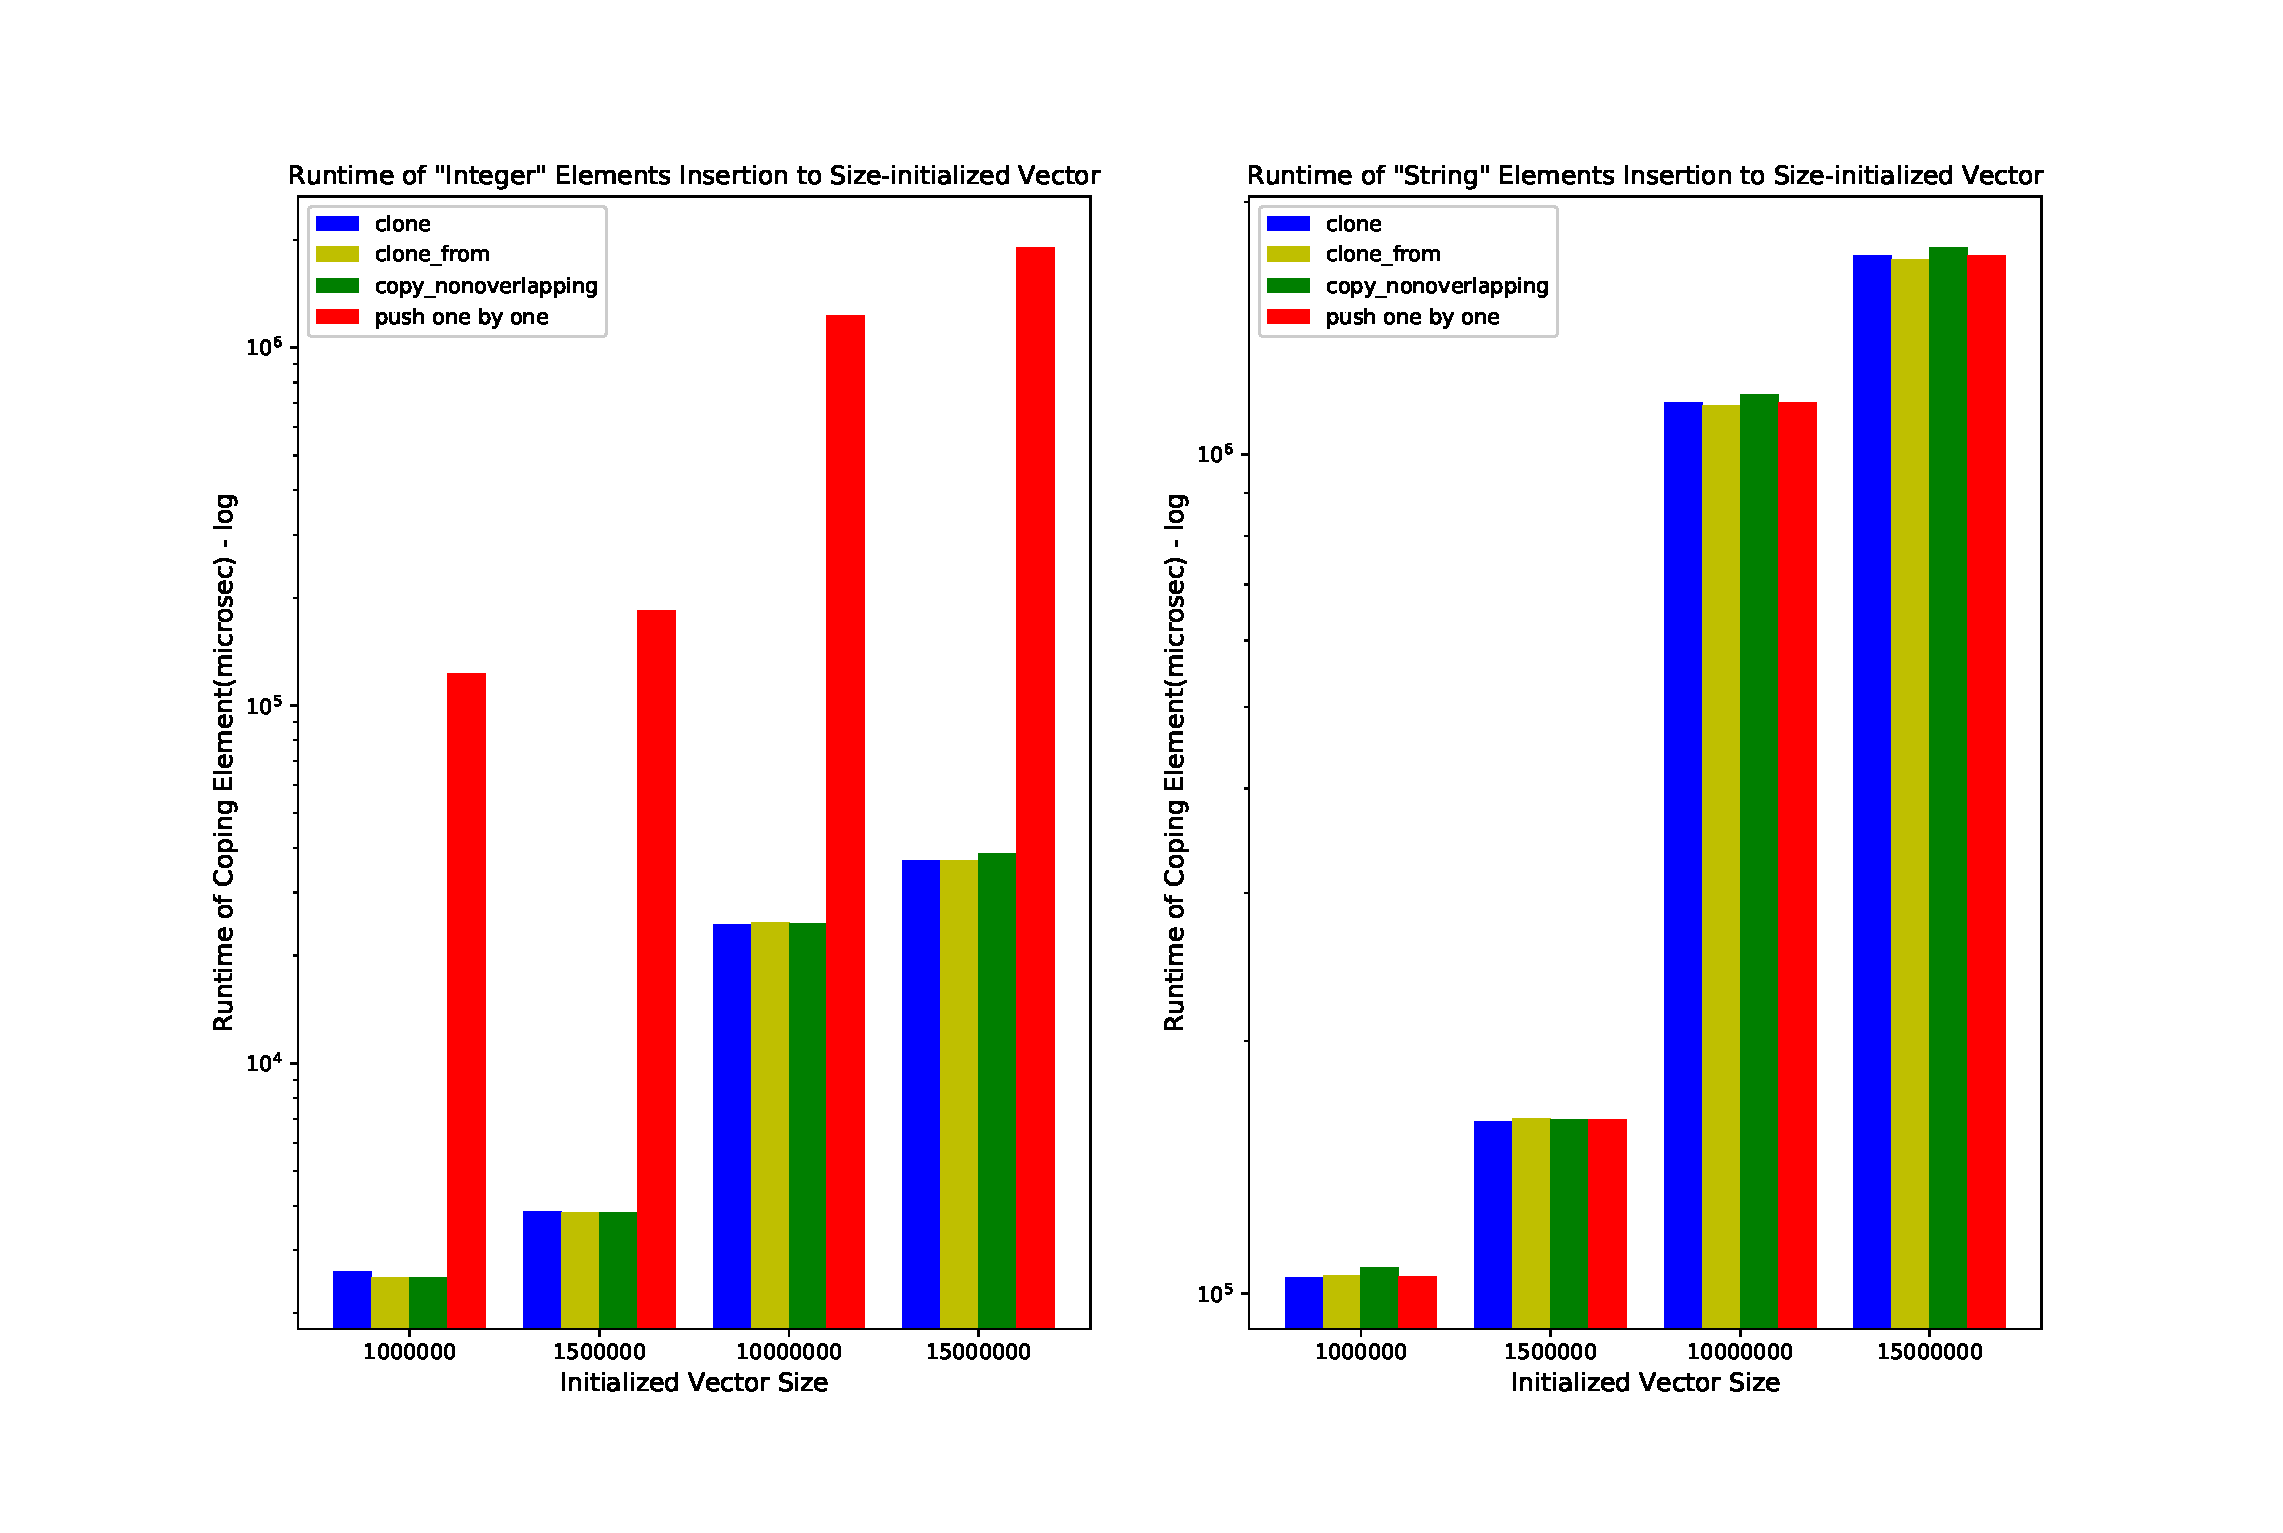
\includegraphics[width=15cm]{rust_various_insertion.eps}
    \caption{Runtime of elements copy from one vector and insertion to the other vector.}
    \label{fig:Sampling}
\end{figure}
\clearpage

\section{Access time to elements in vector}
\label{sec:history}
In this experiment, whether mutability has impacts to operation on the object in terms of runtime performance. 
According to the experiment, there is no difference on accessing to elements of mutable and immutable vector.

\begin{figure}[htb]
    \includegraphics[width=15cm]{rust_various_access.eps}
    \caption{Runtime of elements copy from one vector and insertion to the other vector.}
    \label{fig:Sampling}
\end{figure}

\section{Access time to owned, borrowed, and sliced field of object}
\label{sec:history}
In this experiment, differences of access time to among owned, borrowed, and sliced are observed. 
Each variable has slightly different use of memory. 


\begin{figure}[htb]
    \begin{lstlisting}
        struct CustomerOwned {
            key: i32,
            age: i32,
            num_purchase: i32,
            total_purchase: f64,
            duration_spent: f64, 
            duration_since: f64,
            zip_code: String,
            address: String,
            country: String,
            state: String,
            first_name: String,
            last_name: String,
            province: String,
            comment: String, 
            order: OrderOwned
        }

        struct CustomerBorrowed<'a> {
            key: &'a i32,
            age: &'a i32,
            num_purchase: &'a i32,
            total_purchase: &'a f64,
            duration_spent: &'a f64, 
            duration_since: &'a f64,
            zip_code: &'a String,
            address: &'a String,
            country: &'a String,
            state: &'a String,
            first_name: &'a String,
            last_name: &'a String,
            province: &'a String,
            comment: &'a String, 
            order: &'a OrderBorrowed<'a>
        }

        struct CustomerSlice<'a> {
            key: &'a i32,
            age: &'a i32,
            num_purchase: &'a i32,
            total_purchase: &'a f64,
            duration_spent: &'a f64, 
            duration_since: &'a f64,
            zip_code: &'a str,
            address: &'a str,
            country: &'a str, 
            state: &'a str,
            first_name: &'a str,
            last_name: &'a str,
            province: &'a str,
            comment: &'a str,
            order: &'a OrderSlice<'a>
        }

        struct CustomerRc {
            key: Rc<i32>,
            age: Rc<i32>,
            num_purchase: Rc<i32>,
            total_purchase: Rc<f64>,
            duration_spent: Rc<f64>, 
            duration_since: Rc<f64>,
            zip_code: Rc<String>,
            address: Rc<String>,
            country: Rc<String>,
            state: Rc<String>,
            first_name: Rc<String>,
            last_name: Rc<String>,
            province: Rc<String>,
            comment: Rc<String>, 
            order: Rc<OrderRc>
        }
    \end{lstlisting}
    \caption{Representation of Customer object in Rust.}
    \label{fig:Sampling}
\end{figure}

\clearpage

\begin{figure}[htb]
    \begin{lstlisting}
        struct OrderOwned {
            order_id: i32,
            num_items: i32, 
            payment: f64,
            order_time: f64,
            title: String,
            comment: String
        }


        struct OrderBorrowed<'a> {
            order_id: &'a i32,
            num_items: &'a i32, 
            payment: &'a f64,
            order_time: &'a f64,
            title: &'a String,
            comment: &'a String
        }

        struct OrderRc {
            order_id: Rc<i32>,
            num_items: Rc<i32>, 
            payment: Rc<f64>,
            order_time: Rc<f64>,
            title: Rc<String>,
            comment: Rc<String>
        }
    \end{lstlisting}
    \caption{Representation of Customer object in Rust.}
    \label{fig:Sampling}
\end{figure}

\clearpage



\cleardoublepage

% -------------------------------------
% CHAPTER 3: CONCLUSION
% -------------------------------------
\chapter{Conclusions}
\label{chapter:Conclusions}
\thispagestyle{myheadings}

% set this to the location of the figures for this chapter. it may
% also want to be ../Figures/3_Body/ or something. make sure that
% it has a trailing directory separator (i.e., '/')!
\graphicspath{{3_Conclusion/Figures/}}

% Quick recap of what we did 
% - The purpose of this research
% - Experiment that we conducted
In this thesis, we have presented a number of experiments to assess better implementation of algorithms 
when one develops Big Data analysis tools with Rust programming. 

Difference of variable types does not have impact on operation to access memory address where a value is located. 
This result gives us freedom of choices for variable types to construct complex objects in terms of runtime performance. 
When we however use borrowed types, such as references and slices, their lifetime should be explicitly defined. 
Therefore, we may use owner type variables to construct construct complex objects in order to facilitate lifetime tracking.

Runtime to drop Rc is much 60 times slower than normal reference. This is because Rc needs to check reference count to determine whether to deallocate its value. 
This result may say that we should use normal reference whenever it is possible. 
Again, tracking lifetime of references used in complex objects can be cumbersome. 
Choice of Rc and reference is dependent on complexity of object implemented.

In Rust, we can implement multithread programming with sharing data using Arc. In simple multithread algorithms, 
one can write code where shares data with Arc and simple reference among different threads.
Merge-sort algorithms sharing data with Arc is 21\% slower than normal reference. 
In this situation, sharing data with normal reference require relatively easy lifetime tracking, 
so we should use normal reference to share data among different thread whenever it is possible.

For more complex algorithms, like tree-aggregate and preprocess phase in KNN, one can implement algorithms sharing data with Arc or simply deep-copy the values.
The algorithms with deep-copy is about 40 to 50\% slower than the algorithm with Arc for complex objects.
When we however deal with String, the algorithms with deep-copy is faster than Arc. 
Therefore, the decision which to use deep-copy or Arc method should be determined based on complexity of objects.

Decreasing frequency of memory de/allocation may be an effective solution to improve runtime performance of Big Data processing algorithms. 
There is a trade-off between memory usage and frequency of memory de/allocation. 
That is why developers should conduct careful analysis of algorithms' memory usage pattern and timing of memory de/allocation.

As we can see in the results of experiment, different memory strategy varies the performance of algorithms in Rust programming.
Which memory management strategy to take depends on what objects to deal with. 
Therefore, development of Big Data analysis tools in Rust programming should be started with objects implementation used in the systems.
Next, one can select suitable memory management strategies. 
Finally, algorithms can be optimized with more dedicated strategies to application setting, such as capacity of memory.
\cleardoublepage

%\appendix
\begin{appendices}
\chapter{Proof of xyz}
\label{appendix}
\thispagestyle{myheadings}

\graphicspath{{Appendix/Figures/}}

\section{Memory and Process in Operation Systems}
\label{sec:history}
A process is a section of computation job. A process can work on a CPU core. We can devide process as well.
Basically, each process does not share thier memory. However, for multiprocessing, we could avoid this restriction.
Processes can be represented as tree structure, because a process may create onther child processes.
Process has 4 states, new, running, waiting, and ready. 
Process is represented in process control block (PCB) with state type, process ID, registers, and so on.
The scheduling for process assigning to CPU core is implemented in queues containing PCB. There are two main queues in this scheduler: 
ready queue and wait queue. The head of process in ready queue is selected for execution and once the process requested I/O request or 
production of child process, the running process will be stored n wait queue. Once the request that the process waiting for end, 
the waiting process will be pushed tail of ready queue. 

Processes executing concurrently in the operating system may be either independent processes or cooperating processes excuting in the system.
A process is indepenedent if it does not share data with any other processes. A process cooperating if ti can affect or be affected by the 
other processed executing in the system. In cooperating process, there are two kinds, shared memory and message passing. 
In shared memory, it removes restriction of not interfering memory region. Message passing can be useful for destribution systems as well.

For a pair of processes to communicate throught message, a socket is needed to be established. 
A socket is identified by an IP address concatenated with a port number. When two process communicate, each process will have socket. 
If another process of the same machine wants to communicate, we need new socket to be established. The protocol used in the socket connection
can be TPC and UDP.

\section{Miltithreading and Parallelism}
\label{sec:history}
A thread is a basic unit of CPU usilization, so that a process can have multiple thread. Threads shares mainly code and data. 
Multithreaing is increasingly popular as the multicore programming becomes in common, becasue we can run multiple thread on different core.
Creating thread is much cheaper than creating process and it shares resources so that we do not need addtional methods to allow threads to 
communicate each other, such as sharing memory and message passing.

\section{Memory management in Operation System}
\label{sec:history}
In computer storage hierarchy, the closest strage to CPU is register. It is built into each CPU core and accessible within one cycle of the CPU clock.
However, the same cannot be said of main memory, which is accessed via a transaction on the memory bus. This takes many cycles of the CPU clock.
The remedy is to add fast memeory between the CPU and main memory, typically on the CPU chip for faster access. Such a cache plays a role for this.

For the layout of main memory, it must be ensured that each process has a separate memory space, including operation system. 
The base register and limit register, whose roles are lower boound of memory region and specific size of range respectively, can achieve that goal. 

Usually a program resides on a disk as binary excutable file. To run, the program must be brought into memory and placed within the context of a crocess.
The process is binded to corresponding parts of the physical memory. Binding program to memeory address is staging process. 
There three stages: compile time, load time excution time. The source program is compiled by compiler producing object file. 
After the compilation, the object file is linked with other object file by linker creating executable file . 
Finally, the executable file will be loaded to run execute. At this run time dynamic linbrary link can be done.

If where the process will reside in memory at compile time, absolute code is generated. If this is unknown at the time, 
the binding will be done at load time. At this time, the compiler must generate relocatable code. Otherwise, the binding will be done at 
execution time.

A process does not interact with addresses of physical memory, instead virtual memory. The memory-management unit (MMU) takes roles to map 
logical address to physical address. OS needs to ensure that any of physical memory spaces of processes do not overlap. 
Since one process can be created and deleted and the corresponding memory space should be de/allocated, 
optimization for use of physical memory space is important; we need to allocate memory contiguously avoiding fragmentation.

There are several approaches to deal with this problems. However, we will focus on paging here, which is the most used method OS use to manage memory.
A frame and page are a unit of Separated physical and virtaual memory space in fixed size (4KB or 8KB) respectively.
A process can use as many as pages and correspinding frames obtained by page table matching. This strategy does improve external fragmentation, but not for internal fragmentation.
The smaller size of page has smaller fragmentation, but mapping from page to grame has overhead and also disk I/O is more efficient when the amount of data transfered is larger.



\section{Demand Paging}
\label{sec:history}
A process can have mutiple pages. However, loading entire executable code from sendory storage to memory is not necessarily needed to 
get jobs done. A storategy used in several operating systems is loading only the portion of programs that are needed, demand page. 

In the storatege, some pages currently used are in memory and the others are in secondary storage. 
The page table specifies whether pages are valid or invalid, which means are in memory or not. 
Access to a page marked invalid causes page fault and some steps to resolve the error will be required. 

The first part of process of demand pageing would be that we check an internal table to check whether the reference is valide or invalid.
If the reference is valid, the process reads the content from the memory. Otherwise, we terminates the process and find the free frame in 
physical memory. Then, we schedule a secondary storage operation to read the desired page into newly allocated frame. 
When the storage complete reading the page, we modify the internal table to indicate the page is now in memory. 
Finally, we restart the instruction that was interrupted. 

However, there would be a case where the memory does not have any free frame. In this case, a victim frame that will be replaced with new comming frame should be selected. 
To perform this selection efficiently, a modify bit is tracked for each frame or page. The modify bit represents whether the page is modified since it is loaded from secondary storage. 
If the page or frame is modified, when we swap page we need to update the content in the secondary storage. However, it is not modified, we can simplly delete the frame and replace with new frame.



\section{Copy on Page}
\label{sec:history}
When a parent process creates child process and if these process shares contents on particular page and modify it, 
only the page which has the contenst will be copied.


\section{Threads and Concurrency}
\label{sec:history}

\section{BLAS LAPACK}
\label{sec:history}

Basic Linear Algebra Subprograms (BLAS) are standard building blocks for basic vector and matrix operations. There are 3 levels of operation. The level 1 BLAS performs scalar, 
vector and vector-vector operations, the level 2 BLAS performs matrix-vector operation, and the level 3 BLAS performs matrix-matrix operation. 

LAPACK is developed on BLAS and has advanced functionalities such as LU decomposition and Singular Value Decomposition (SVD). Dense and banded matrices are handled, but not general 
sparse matrices. The initial motivation of development of LAPACK was to make the widely used EISPACK and LINPACK libraries run efficiently on shared-memory vector and parallel processors. 
LINPACK and EISPACK are inefficient because their memory access patterns disregard the multi-layered memory hierarchies of the machines, thereby spending too much time moving data. 
LAPACK addresses this problem by recognizing the algorithms to use block matrix operations, such as matrix multiplication, in the innermost loops. These block operations can be optimized for each architecture to account for the memory hierarchy, 
and so provide a portable way to achieve high efficiency on diverse modern machines. However, LAPACK requires that highly optimized block matrix operations be already implemented on each machine. 

ARPACK is also a collection of linear algebra subroutines which is designed to compute a few eigenvalues and corresponding eigenvectors from large scale matrix. 
ARPACK is based upon an algorithmic variant of the Arnoldi process called the Implicitly Restarted Arnoldi Method (IRAM). 
When the matrix is symmetric it reduces to a variant of the Lanczos process called the Implicitly Restarted Lanczos Method(IRLM). The Arnoldi process only interacts with the matrix via matrix-vector multiplies. 
Therefore, this method can be applied to distributed matrix operations required in big data analysis.


The original BLAS and LAPACK are written in Fortran90. Linear algebra library used for Spark is netlib-java, which is a Java wrapper library for Netlib, C API of BLAS and LAPACK. 
The reason why the developers addressed to use this package is that the BLAS and LAPACK are already bug free and implementing linear algebra library from scratch can usually buggy. 

However, the main advantage of use of BLAS and LAPACK is system optimized implementation. So if we implement original Fortran linear algebra library, it cannot perform as well as BLAS and LAPACK. 
And the performance would not be such different from one of implementation in Java or Rust.  If we want to test only memory management between Rust and Java, 
it can be enough implementation of linear algebra operation from  pure Java and Rust sacrificing the best performance taking advantage of system optimization. 


\section{Netlib-Java}
\label{sec:history}

Netlib-java is a Java wrapper of BLAS, LAPACK, and ARPACK. Netlib-java choose  implementation of linear algebra depending on installation of the libraries. 
First, if we have installed machine optimised system libraries, such as Intel MKL and OpenBLAS, netlib-java will use these as the implementation to use. 
Next, it try to load netlib references which netlib-java use CBLAS and LAPCKE interface to perform BLAS and LAPACK native call. 
The last option is to use f2j which is intended to translate the BLAS and LAPACK libraries from their Fortran77 reference source code to Java class files, 
instead of calling native libraries by using Java Native Interface (JNI). 

We can use JNI to call native libraries from Java. The JNI is a native programming interface which allows Java code that runs inside a Java Virtual Machine (VM) 
to interoperate with applications and libraries written in other programming languages. 

\section{Create Java interface of CBLAS with JNI}
\label{sec:history}
\begin{enumerate}
    \item Download BLAS and build using make file. In the figure2.1, the built file is libblas.a and the header file is blas.h.
    \item Download CBLAS and build using make file (I am not sure whether we should build archive file or shared library). In figure, the build file would be libcblas.a or libcblas.dylib and header file is cblas.h.
    \item Create java file which will be the Java interface of CBLAS.
    \item Compile java file with -h header flag to create class file (CBLASJ.class) and header file (CBLASJ.h).
\begin{lstlisting}[language=bash]
    $ javac -h . CBLASJ.java
\end{lstlisting}
    \item Create C file (CBLASJ.c) which will bind Java interface and CBLAS library. And compile it with JNI to create object file (CBLASJ.o).
\begin{lstlisting}[language=bash]
    $ gcc -c-fPIC -I${JAVA_HOME}/include -I${JAVA_HOME}/include/darwin CBLASJ.c
\end{lstlisting}
    \item Compile shared library linking library (libcblas.a or libcblas.dylib) object file (CBLASJ.o).
\begin{lstlisting}[language=bash]
    $ gcc -o libcblas.dylib (or libcblas.a) CBLASJ.o 
\end{lstlisting}
\end{enumerate}

\begin{figure}[htb]
    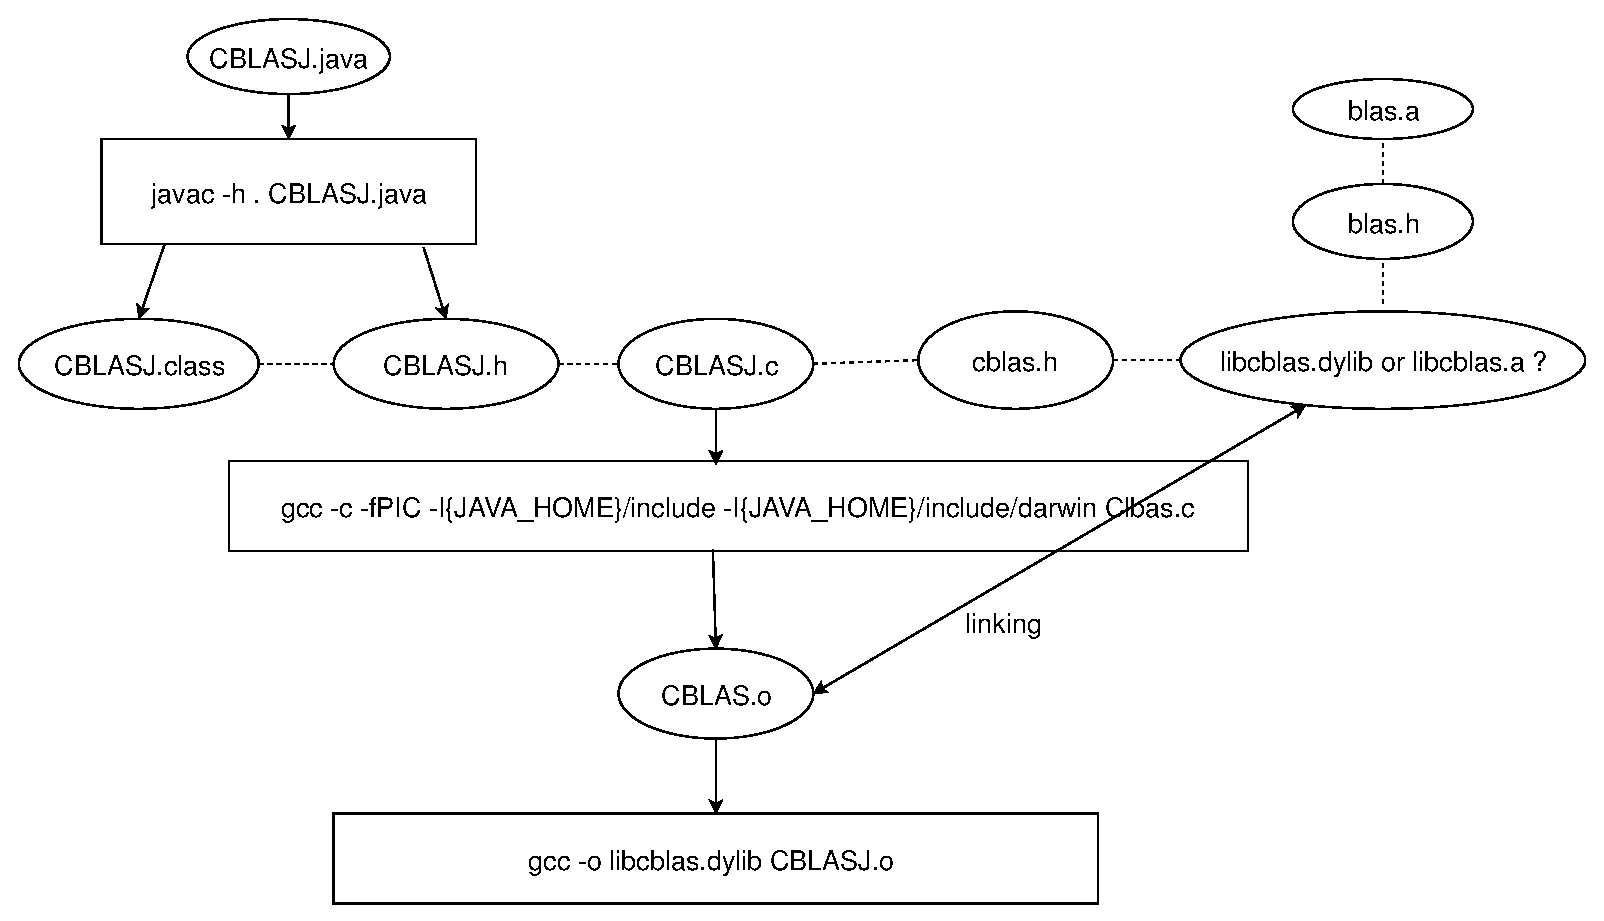
\includegraphics[width=15cm]{cblas_with_jni.eps}
    \caption{Integration of Native Methods }
    \label{fig:Sampling}
\end{figure}



\section{Matrix Computation and Optimization in Apache Spark}
\label{sec:history}

Matrix operation is a fundamental part of machine learning. Apache Spark provides implementation for distributed and local matrix operation. 
To translate single-node algorithms to run on a distributed cluster, Spark addresses separating matrix operations from vector operations and run matrix operations on the cluster, 
while keeping vector operations local to the driver. 

Spark changes its behavior for matrix operations depending on the type of operations and shape of matrices. For example, Singular Value Decomposition (SVD) for a square matrix is performed in distributed cluster, 
but SVD for a tall and skinny matrix is on a driver node. This is because the matrix derived among the computation of SVD for tall and skinny matrix is usually small so that it can fit to single node.

Spark uses ARPACK to solve square SVD. ARPACK is a collection of Fortran77 designed to solve eigenvalue problems. ARPACK is based upon an algorithmic variant of the Arnoldi process called the Implicitly Restarted Arnoldi Method (IRAM). 
When the matrix A is symmetric it reduces to a variant of the Lanczos process called the Implicitly Restarted Lanczos Method (IRLM). 
ARPACK calculate matrix multiplication by performing matrix-vector multiplication. So we can distribute matrix-vector multiplies, and exploit the computational resources available in the entire cluster. 
The other method to distribute matrix operations is Spark TFOCS. Spark TFOCS supports several optimization methods.

To allow full use of hardware-specific linear algebraic operations on single node, Spark uses the BLAS (Basic Linear Algebra Systems) interface with relevant libraries for CPU and GPU acceleration. 
Native libraries can be used in Scala are ones with C BLAS interface or wrapper and called through the Java native interface implemented in Netlib-java library and wrapped by the Scala library called Breeze. 
Following is some of the implementation of BLAS.

\begin{itemize}
    \item f2jblas -  Java implementation of Fortran BLAS
    \item OpenBLAS - open source CPU-optimized C implementation of BLAS
    \item MKL - CPU-optimized C and Fortran implementation of BLAS by Intel
\end{itemize}

These have different implementation and they perform differently for the type of operation and matrices shape. 
In Sark, OpenBlas is the default method of choice. BLAS interface is made specifically for dense linear algebra. 
Then, there are few libraries that efficiently handle sparse matrix operations.

\section{Memory Management of each Linear Algebra Library}
\label{sec:history}

The pure Java linear algebra library, such as La4j, EJML, and Apache Common Math, 
use normal GC performed by JVM to manage memory. This is because the implementation of these libraries are in purely Java.

Netlib-java, Jblas or other simple Java wrapper of BLAS, LAPACK, and ARPACK with Java Native Interface (JNI) use normal GC as well. 
This is because the native code deals with Java array by obtaining a reference to it. After the operation, 
the native method releases the reference to the Java array with or without returning new Java array or Java primitive type object. 

ND4J has two types of  its own memory management methods, GC to pointer of off-heap NDArray, and MemoryWorkspaces. 
ND4J used off-heap memory to store NDArrats, to provide better performance while working with NDArrays from vative code such as BLAS and CUDA libraries. 
Off-heap means that the memory is allocated outside of the Java heap so that it is not managed by the JVM’s GC. NDArray itself is not tracked by JVM, 
but its pointer is. The Java heap stores pointer to NDArray on off-heap. When a pointer is dereferenced, this pointer can be a target of JVM’s GC and when it is collected, 
the corresponding NDArray will be deallocated. When using MemoryWorkspaces, NDArray lives only within specific workspace scope. 
When NDArray leaves the workspace scope, the memory is deallocated unless explicitly calling method to copy the NDArray out of the scope.

\end{appendices}
%==========================================================================%
% Bibliography
\newpage
\singlespace
\bibliographystyle{acm}

% each subdirectory can have its own BiBTeX file
\bibliography{thesis}
\cleardoublepage

%==========================================================================%
% Curriculum Vitae
\addcontentsline{toc}{chapter}{Curriculum Vitae}
\thispagestyle{empty}


\begin{center}
{\LARGE {\bf CURRICULUM VITAE}}\\
\vspace{0.5in}
\end{center}

\setcounter{section}{0}
\renewcommand*{\theHsection}{chX.\the\value{section}}

\section*{Contact}
\begin{itemize}
    \item Phone: +81-90-4148-4639 \textbullet{} City: Tokyo \textbullet{} Email: \href{golisaku4639@gmail.com}{golisaku4639@gmail.com} 
    \item GitHub: \href{https://github.com/ShinsakuOkazaki}{\textbf{github}.com/ShinsakuOkazaki} 
    \item LinkedIn\href{https://www.linkedin.com/in/shinsaku-okazaki-7b786b13b}{ \textbf{linkedin}.com/in/shinsaku-okazaki-7b786b13b}
\end{itemize}

\section*{Education}
\subsection*{Boston University, Boston, MA}
\begin{itemize}
    \item Program: Master of Science in Computer Information Systems (September 2018 - May 2020)
    \item Course Work: Software Design Pattern, Database, Big Data Analysis, Data Analysis
    \item Master Thesis: An Experimental Study of Memory Management with Rust Programming for Big Data Processing
\end{itemize}

\subsection*{Seikei University, Tokyo}
\begin{itemize}
    \item Program: Bachelor of Science in System Design (April 2013 - March 2018)
    \item Course Work: Image Processing, Control Engineering, Digital Signal Processing, Engineering Economics
\end{itemize}


\section*{Experience} 
\subsection*{Research Assistant, Boston University, September 2019 - May 2020}
\begin{itemize}
    \item  Improved run-time performance of Large Scale Sort Algorithm 30\% by implementing algorithm with careful Memory Management strategies in Rust.
    \item  Developed Merge-sort Algorithm and Tree-aggregate Algorithm with Multithreading using Rust on Cloud Instances using GCP.
    \item Implemented \textbf{Machine Learning} Algorithm with different memory management strategy to assess best workflow on \textbf{Natural Language Processing} with Rust.
\end{itemize}

\subsection*{Teaching Assistant, Boston University, September 2019 - May 2020}
\begin{itemize}
    \item  Developed a R package where student can take R programming exercises to improve student's learning experience.
    \item  Designed data collection feature by adding REST APIs using Flask and MongoDB.
    \item  Facilitated customization of software by reducing building process 60\% with automation using Bash script.
    \item  Collaborated with a team of 4 members to design flexible and robust software architecture.
\end{itemize}

\subsection*{Software Engineer Intern, Brigham and Women's Hospital, June 2019 - August 2019}
\begin{itemize}
    \item  Automated data inputs with attribute suggestion feature using React.js and AJAX
    \item  Designed data collection feature by adding REST APIs using Flask and MongoDB.
    \item  Wrote about 100 unit test cases in Mocha and Chai and increased test coverage by 5\%.
\end{itemize}





	
 

%==========================================================================%
\end{document}
